\section*{Introduction}
\addcontentsline{toc}{section}{Introduction}
Properly regularize machine with flexible junctions (see \small{Figure~\ref{fig:ejexample}}) is not a toy problem. As a matter of fact, the presence of elasticity at joint level is very common in industrial robots that heavily relies on motion transmission/reduction elements such as: belts, long shafts, cables, harmonic drives, or cycloidal gears Figure~\ref{fel}; aiming to relocate the actuators next to the robot base, thus improving power/dynamic efficiency. Flexible elements are also preferred for physical human–robot interaction, since they allow a decoupling between actuators and the lighter links. As always there is a trade-off: increasing the agility and safety of the robot we pay a cost in controlling it with a more complex and sophisticated law. Therefore many different approaches have been proposed \cite{simplepd,deluca93,deluca96} and in what follow we'll report our reasoning and experiments applying the learning one \cite{deluca96} adapted to our study case, underling the differences with respect to the rigid model studied during the course and giving a proof of convergence as well.

\begin{figure}[h!]
\centerline{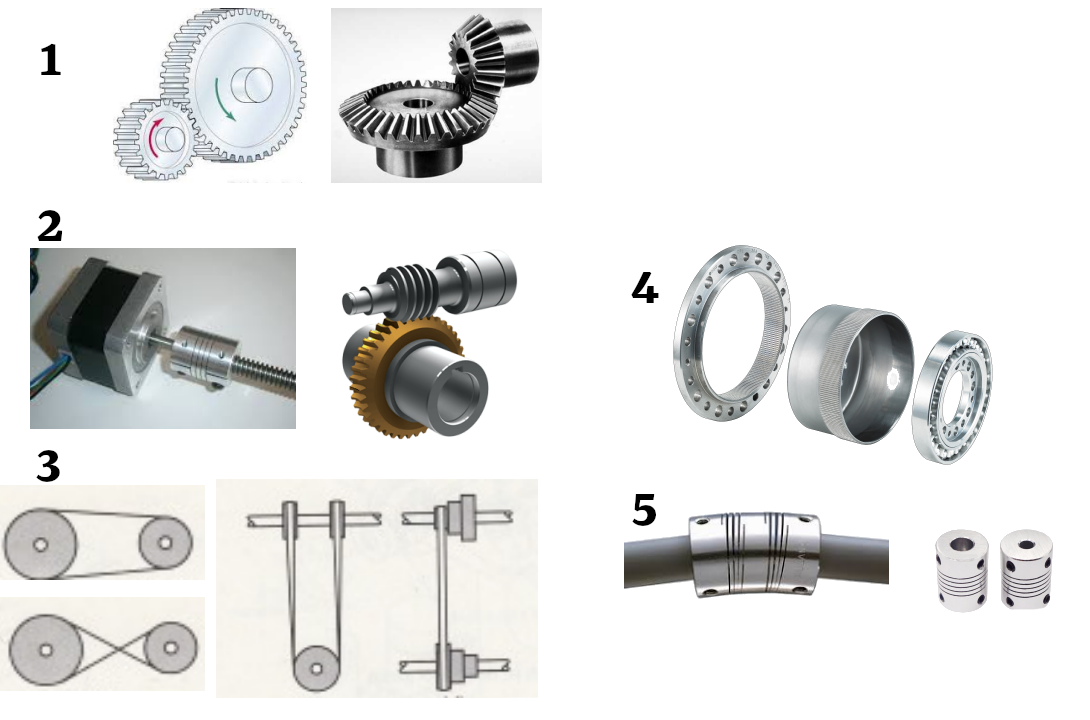
\includegraphics[scale=1]{figures/flexelements.png}}
\caption{\label{fel}
Some of the most common transmissions: 1) spur gears, 2) lead screws \& worm gearing, 3)
toothed belts \& chains, 4) harmonic drives, 5) transmission shafts.}
\end{figure}

\begin{center}
\begin{figure}[h]
\begin{minipage}[b]{0.45\linewidth}
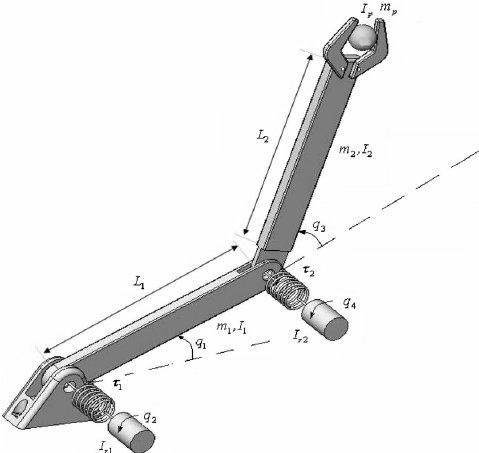
\includegraphics[scale=0.3]{figures/Two-Link-Flexible-Joint-Robot-Manipulator_W640.jpg}
\caption{Example of a two-link flexible joint robot Manipulator.}
\label{fig:ejexample}
\end{minipage}
\hspace{0.5cm}
\begin{minipage}[b]{0.45\linewidth}
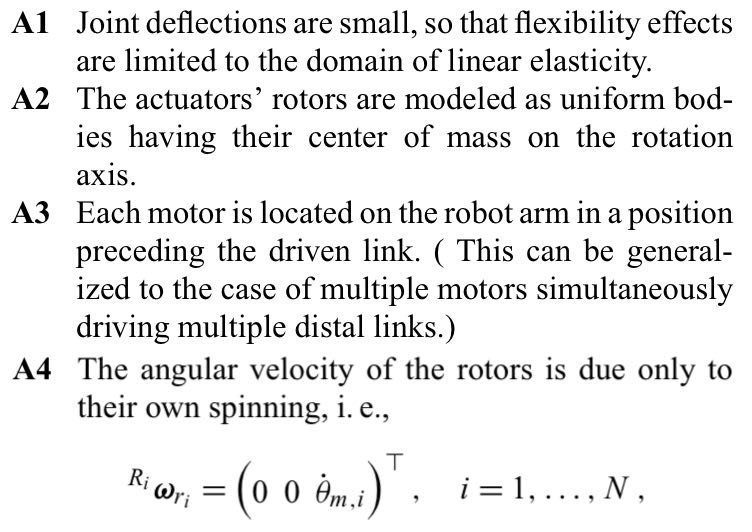
\includegraphics[width=\textwidth]{figures/assumptions.jpg}
\caption{Standard assumptions made for modelling a robot with its elasticity.}
\label{fig:assumpt}
\end{minipage}
\end{figure}
\end{center}

% \begin{figure}[h!]
% \centerline{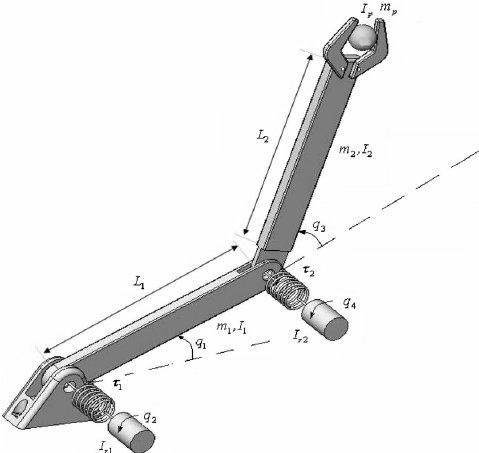
\includegraphics[scale=0.3]{figures/Two-Link-Flexible-Joint-Robot-Manipulator_W640.jpg}}
% \caption{\label{elr}
% Example of a Two-Link Flexible Joint Robot Manipulator. \\\small{Picture taken from Ali Alamdari on researchgate.}}
% \end{figure}
